\vspace{10pt}

{\centering\subsection*{何梓萌:爱唠叨的妈妈}}

\addcontentsline{toc}{subsection}{何梓萌:爱唠叨的妈妈}

\renewcommand{\leftmark}{何梓萌:爱唠叨的妈妈}

\begin{figure}[htbp]

\centering

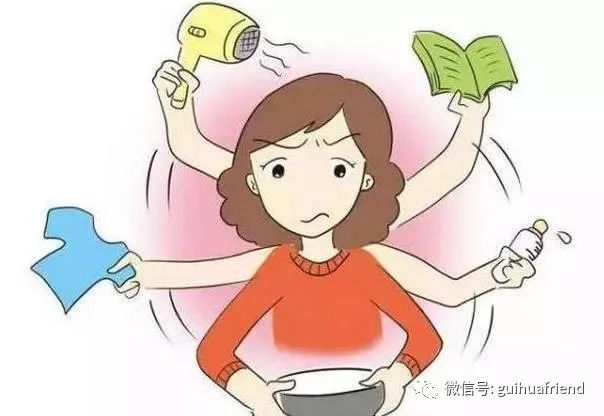
\includegraphics[width = .5\textwidth]{./ch/10.jpg}

\end{figure}



我的妈妈,她特别爱唠叨。她长着一头乌黑的长发,长得眉清目秀,头像一个大西瓜。两只葡萄大的眼睛,看起来炯炯有神。两条像柳叶弯的眉毛,黑得舒服,黑得发亮。一张能说会道的樱桃小嘴,然后就是这么一个家庭主妇,却很唠叨,不信你看:

有一天,已经非常晚了,我累得像狗,弯着腰,有气无力地走回家,一回家,我就把鞋随地一扔,直接把书包丢在沙发上,躺在沙发上看着电视。妈妈看到了我,火冒三丈地说:“你这是干什么了?鞋子随地乱扔,书包直接丢在沙发上,你个女孩子不能矜持一点吗?”我听着这些像唐僧在念经一样,迷糊了起来,然后灰溜溜地跑走了。

还有一次,我正在房间里看书,妈妈忽然走过来,皱着眉,脸红彤彤地说:“你这个房间,乱的像个猪窝,你就不能收拾一下,还有你这个地,这么多垃圾,不能扫一下吗?你的书包脏死了,快去河边洗一下!”说完,妈妈就拉着我去河边,我第一次干这事,笨手笨脚的,妈妈看到了就怒气冲冲,跺着脚,指着我说:“这点小事都干不好,长大了该怎么办?快点洗!”周围人都吓死了,他们非常惊讶,有些小孩子都吓哭了。

还有一次,我生了场大病,我非常虚弱,嘴巴白白干干的。妈妈很生气地说:“看,都是你不盖被子,才变成这样,下次不许了!”说完,就起身去给我冲药了。我喝完了药,一睡就睡到了第二天早上。早上,我起来就看到了妈妈在我旁边,她看到我醒了,就问我:“宝贝,还疼不疼,病好了吗?”她紧紧抱住我,我看起来好多了,妈妈也去给我做早餐了。我很疑惑,为什么妈妈在我旁边。我百思不得其解,我赶忙跑去找爸爸,爸爸告诉了我真实情况,原来妈妈不放心,怕再踢被子,我就一直不好,所以我妈妈才会一直守在我床边,我知道了就哭了。

这一刻,我明白了所有,原来妈妈对我们的唠叨是对我们的爱,对我们好。从此,我就不觉得妈妈的唠叨很烦。我爱你,妈妈!





\vspace{10pt}



作者:五(3)班 何梓萌



指导老师:刘婷



投稿:2021年6月3日





发表:2021年6月4日






                



\vspace{10pt}

\hline



